\documentclass[a4paper]{article}
\usepackage{times}
\usepackage[utf8]{inputenc}
\usepackage{selinput}
\usepackage{upquote}
\usepackage[margin=2cm, rmargin=4cm, tmargin=3cm]{geometry}
\usepackage{tcolorbox}
\usepackage{xspace}
\usepackage[french]{babel}
\usepackage{url}
\usepackage{hyperref}
\usepackage{fontawesome5}
\usepackage{marginnote}
\usepackage{ulem}
\usepackage{tcolorbox}
\usepackage{graphicx}
%\usepackage[top=Bcm, bottom=Hcm, outer=Ccm, inner=Acm, heightrounded, marginparwidth=Ecm, marginparsep=Dcm]{geometry}


\newtcolorbox{Example}[1]{colback=white,left=20pt,colframe=slideblue,fonttitle=\bfseries,title=#1}
\newtcolorbox{Solutions}[1]{colback=white,left=20pt,colframe=green,fonttitle=\bfseries,title=#1}
\newtcolorbox{Conseils}[1]{colback=white,left=20pt,colframe=slideblue,fonttitle=\bfseries,title=#1}
\newtcolorbox{Warning}[1]{colback=white,left=20pt,colframe=warning,fonttitle=\bfseries,title=#1}

\setlength\parindent{0pt}

  %Exercice environment
  \newcounter{exercice}
  \newenvironment{Exercice}[1][]
  {
  \par
  \stepcounter{exercice}\textbf{Question \arabic{exercice}:} (\faClock \enskip \textit{#1})
  }
  {\bigskip}
  

% Title
\newcommand{\titre}{\begin{center}
  \section*{Algorithmes et Pensée Computationnelle}
\end{center}}
\newcommand{\cours}[1]
{\begin{center} 
  \textit{#1}\\
\end{center}
  }


\newcommand{\exemple}[1]{\newline~\textbf{Exemple :} #1}
%\newcommand{\attention}[1]{\newline\faExclamationTriangle~\textbf{Attention :} #1}

% Documentation url (escape \# in the TP document)
\newcommand{\documentation}[1]{\faBookOpen~Documentation : \href{#1}{#1}}

% Clef API
\newcommand{\apikey}[1]{\faKey~Clé API : \lstinline{#1}}
\newcommand{\apiendpoint}[1]{\faGlobe~Url de base de l'API \href{#1}{#1}}

%Listing Python style
\usepackage{color}
\definecolor{slideblue}{RGB}{33,131,189}
\definecolor{green}{RGB}{0,190,100}
\definecolor{blue}{RGB}{121,142,213}
\definecolor{grey}{RGB}{120,120,120}
\definecolor{warning}{RGB}{235,186,1}

\usepackage{listings}
\lstdefinelanguage{texte}{
    keywordstyle=\color{black},
    numbers=none,
    frame=none,
    literate=
           {é}{{\'e}}1
           {è}{{\`e}}1
           {ê}{{\^e}}1
           {à}{{\`a}}1
           {â}{{\^a}}1
           {ù}{{\`u}}1
           {ü}{{\"u}}1
           {î}{{\^i}}1
           {ï}{{\"i}}1
           {ë}{{\"e}}1
           {Ç}{{\,C}}1
           {ç}{{\,c}}1,
    columns=fullflexible,keepspaces,
	breaklines=true,
	breakatwhitespace=true,
}
\lstset{
    language=Python,
	basicstyle=\bfseries\footnotesize,
	breaklines=true,
	breakatwhitespace=true,
	commentstyle=\color{grey},
	stringstyle=\color{slideblue},
  keywordstyle=\color{slideblue},
	morekeywords={with, as, True, False, Float, join, None, main, argparse, self, sort, __eq__, __add__, __ne__, __radd__, __del__, __ge__, __gt__, split, os, endswith, is_file, scandir, @classmethod},
	deletekeywords={id},
	showspaces=false,
	showstringspaces=false,
	columns=fullflexible,keepspaces,
	literate=
           {é}{{\'e}}1
           {è}{{\`e}}1
           {ê}{{\^e}}1
           {à}{{\`a}}1
           {â}{{\^a}}1
           {ù}{{\`u}}1
           {ü}{{\"u}}1
           {î}{{\^i}}1
           {ï}{{\"i}}1
           {ë}{{\"e}}1
           {Ç}{{\,C}}1
           {ç}{{\,c}}1,
    numbers=left,
}

\newtcbox{\mybox}{nobeforeafter,colframe=white,colback=slideblue,boxrule=0.5pt,arc=1.5pt, boxsep=0pt,left=2pt,right=2pt,top=2pt,bottom=2pt,tcbox raise base}
\newcommand{\projet}{\mybox{\textcolor{white}{\small projet}}\xspace}
\newcommand{\optionnel}{\mybox{\textcolor{white}{\small Optionnel}}\xspace}
\newcommand{\advanced}{\mybox{\textcolor{white}{\small Pour aller plus loin}}\xspace}
\newcommand{\auto}{\mybox{\textcolor{white}{\small Auto-évaluation}}\xspace}


\usepackage{environ}
\newif\ifShowSolution
\NewEnviron{solution}{
  \ifShowSolution
	\begin{Solutions}{\faTerminal \enskip Solution}
		\BODY
	\end{Solutions}
  \fi}


  \usepackage{environ}
  \newif\ifShowConseil
  \NewEnviron{conseil}{
    \ifShowConseil
    \begin{Conseils}{\faLightbulb \quad Conseil}
      \BODY
    \end{Conseils}

    \fi}

    \usepackage{environ}
  \newif\ifShowWarning
  \NewEnviron{attention}{
    \ifShowWarning
    \begin{Warning}{\faExclamationTriangle \quad Attention}
      \BODY
    \end{Warning}

    \fi}
  

%\newcommand{\Conseil}[1]{\ifShowIndice\ \newline\faLightbulb[regular]~#1\fi}


\usepackage{array}
\usepackage{amsmath}
\usepackage{amssymb}
\usepackage{tabto}
\usepackage{subfigure}
\newcolumntype{C}[1]{>{\centering\let\newline\\\arraybackslash\hspace{0pt}}m{#1}}

\begin{document}

% Change the following values to true to show the solutions or/and the hints
\ShowSolutiontrue
\ShowConseiltrue
\ShowNotefalse
\ShowDessintrue
\titre
\cours{Algorithmes probabilistes}

Le but de cette séance est de comprendre les algorithmes probabilistes. Ceux-ci permettent de résoudre des problèmes complexes en relativement peu de temps. La contrepartie est que le résultat obtenu est généralement une solution approximative du problème initial. Néanmoins, ces algorithmes demeurent très utiles pour beaucoup d'applications.

\section{Monte-Carlo}
\begin{Exercice}[10 minutes]\textbf{Un jeu de hasard : Python}\\
    Supposez que vous lanciez une pièce de monnaie \textbf{l} fois et que vous voulez calculez la probabilité d'avoir un certain nombre de piles. Vous devez programmer un algorithme probabiliste, permettant de calculer cette probabilité. Pour ce faire, vous devez compléter la fonction \textit{proba(n,l,iter)} contenue dans le fichier \lstinline{Piece.py} (Dans le dossier \lstinline{Code}). La fonction \textit{Piece(l)} permet de créer une liste contenant des 0 et des 1 aléatoirement avec une probabilité $\frac{1}{2}$. Considérez un chiffre 1 comme une réussite (pile) et 0 comme un échec (face).
    \\
    \begin{conseil}
     \begin{enumerate}
            \item Pour estimer empiriquement la probabilité d'un événement, comptez le nombre de fois que l'événement en question se produit en effectuant un nombre d'essais. Puis divisez le nombre d'occurrences de l'événement par le nombre total d'essais. Par exemple, si vous voulez estimer la probabilité d'obtenir un 2 avec un dé. Lancez le dé 1000 fois, comptez le nombre de fois que vous obtenez 2, et divisez le résultat par 1000.
        \item La méthode \lstinline{random.randint(début, fin)} contenue dans la fonction \lstinline{piece} permet de choisir de façon aléatoire un nombre dans un intervalle.
    \end{enumerate}
    \end{conseil}
    \begin{solution}
        \lstinputlisting[language = python]{solutions/Piece_correction.py}
    \end{solution}
    \end{Exercice}


\begin{Exercice}[15 minutes]\textbf{Une approximation de $\pi$ : Python}\\
    L'objectif de cet exercice est d'écrire un algorithme probabiliste permettant d'approximer le nombre $\pi$. Imaginez un plan sur lequel $0 \leq x \leq 1$ et $0 \leq y \leq 1$. Sur ce dernier, nous allons dessiner un quart de cercle centré en (0,0) et avec un rayon de 1. Par conséquent, un point dans cet espace se trouve à l'intérieur ou sur le cercle si $x^2 + y^2 \leq 1$. Vous trouverez ci-dessous une illustration de la situation:
    
    La première étape de cet exercice consiste à créer une fonction permettant de déterminer si un point est à l'intérieur (zone rouge) ou à l'extérieur du cercle. Puis, générez 10000 points dans cet espace (x et y devraient appartenir à l'intervalle [0,1]). Pour ce faire, vous pouvez utliser la fonction \textit{random.random()} après avoir importé le module \textbf{random}. Vous pouvez obtenir l'approximation de $\pi$ à partir de la formule suivante : $\pi \approx (\frac{\text{Nombre de points dans le cercle}}{\text{Nombre total de points}})\cdot 4$. Votre réponse devrait être assez proche de la vraie valeur de $\pi$.\\
    
    \begin{conseil}
        La fonction \lstinline{random.random()} génère aléatoirement un chiffre compris entre 0 et 1. Etant donné que vous devez simuler des points en 2 dimensions, vous devrez utiliser 2 fois cette fonction.
    \end{conseil}
    \begin{center}
        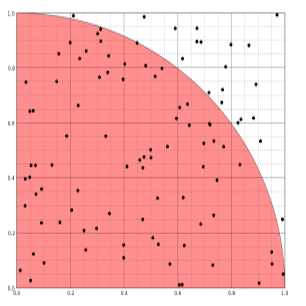
\includegraphics[]{resources/Cercle.PNG}
    \end{center}
    \begin{solution}
        \lstinputlisting[language = python]{solutions/Pi.py}
    \end{solution}
    
\end{Exercice}

\section{Fingerprinting}
\begin{Exercice}[15 minutes]\textbf{Fingerprinting: Une mission pour l'agente secrète Alice: Python}\\
    Dans cet exercice, vous prendrez le rôle de l'agente secrète Alice. Cette dernière enquêtait sur la disparition de son collègue,
    l'agent Bob, et se doutait que l'indice clé qui la mènerait à la vérité se trouvait dans la boîte mail de Bob. Alice arriva à trouver
    un bout de papier avec écrit dessus : ``\textit{Mon mot de passe est l'empreinte de ceciestmonmotdepasse}''. Aidez Alice à trouver l'empreinte du mot de passe! \\

    Pour cela, vous devez compléter deux fonctions :
    \begin{enumerate}
        \item \lstinline{is_a_prime_number(num)} qui vérifie que \lstinline{num} est un nombre premier ou pas. Un nombre premier est un entier naturel 
        qui admet exactement deux diviseurs distincts entiers et positifs. Ces deux diviseurs sont 1 et le nombre considéré, 
        puisque tout nombre a pour diviseurs 1 et lui-même, les nombres premiers étant ceux qui n’en possèdent aucun autre.
        
        \item \lstinline{fingerprinting(p, message)} qui implémente l'algorithme de fingerprinting suivant :
              \begin{enumerate}
                  \item Si \lstinline{p} est un nombre premier, calculez la valeur de hachage de la chaîne à l'aide de la fonction \lstinline{hash(...)}, puis calculez le modulo du résultat du hachage avec \lstinline{p}.
                  \item Sinon, affichez un message qui dit que le nombre n'est pas un nombre premier.    
              \end{enumerate}
    \end{enumerate}

    Si vous réussissez à implémenter les deux fonctions correctement, le programme vous affichera : \lstinline{Connexion réussie? True}.

    À vos ordis, détectives!

    \lstinputlisting[language = python]{resources/fingerprinting.py}
\begin{conseil}
Le code ci-dessus se trouve sur Moodle, dans le dossier \lstinline{Code>fingerprinting.py}.\\
Pour vérifier si un nombre $n$ est premier, il faut  parcourir tous les nombres à partir de $2$~à~$(n//2+1)$ et vérifier si chaque nombre divise $n$. Si un nombre qui divise $n$ est trouvé, il faut retourner \lstinline{False}. Si aucun diviseur est trouvé alors cela signifie que $n$ est premier et il faut retourner \lstinline{True}.
\end{conseil}

    \begin{solution}
        \lstinputlisting[language = python]{solutions/fingerprinting_solution.py}
    \end{solution}
\end{Exercice}

\newpage
\section{Las Vegas}

\begin{Exercice}[10 minutes]\textbf{Un point dans un cercle unitaire : Python} \optionnel\\
    Les algorithmes de Monte Carlo sont des algorithmes probabilistes dont la sortie peut être incorrecte avec une certaine probabilité, qui est généralement faible. En revanche, un algorithme de Las Vegas est un algorithme probabiliste qui trouve toujours le bon résultat lorsqu'il existe. Son inconvénient est que sa complexité temporelle ne peut être garantie à l'avance car elle dépend des données passées en paramètres.\\ \\
    L'objectif de cet exercice est d'écrire un algorithme probabiliste permettant de générer les coordonnées d'un point contenu dans un cercle unitaire. Pour cela, vous pouvez générer des points \lstinline{n} fois jusqu'à ce que vous trouviez un point qui soit contenu dans le cercle.
    
    
    donner un point contenu dans un cercle unitaire. 
    
    \begin{conseil}
       Vous pouvez vous inspirer de l'exercice 2 \textit{(Approximation de $\pi$ )}.
    \end{conseil}
    \begin{solution}
     \lstinputlisting[language = python]{solutions/LV_Point.py}
    \end{solution}
    \end{Exercice}

\begin{Exercice}[20 minutes] \textbf{Quicksort - Algorithme de Las Vegas: Python}\\
    Dans cet exercice, vous allez implémenter un algorithme de tri rapide (quicksort) sur une liste d'éléments avec l'algorithme de Las Vegas.
\\\\
    L'algorithme de tri rapide applique un paradigme \textit{divide-and-conquer} afin de trier un ensemble de nombres~\lstinline{A}. Il fonctionne en trois étapes: 
    \begin{enumerate}
        \item il choisit d'abord un élément pivot, \lstinline{A[q]}, en utilisant un générateur de nombres aléatoires (d'où sa nature d'algorithme dit probabiliste) ;
        \item puis il réorganise le tableau en deux sous-tableaux $A[p...q-1]$ et $A[q+1...r]$, où les éléments des premier et deuxième tableaux sont respectivement plus petits et plus grands que $A[q]$.
        \item L'algorithme applique ensuite récursivement les étapes de tri rapide ci-dessus sur les deux tableaux indépendants, produisant ainsi un tableau entièrement trié.\\
    \end{enumerate}
    \begin{figure}[h]
        \centering
        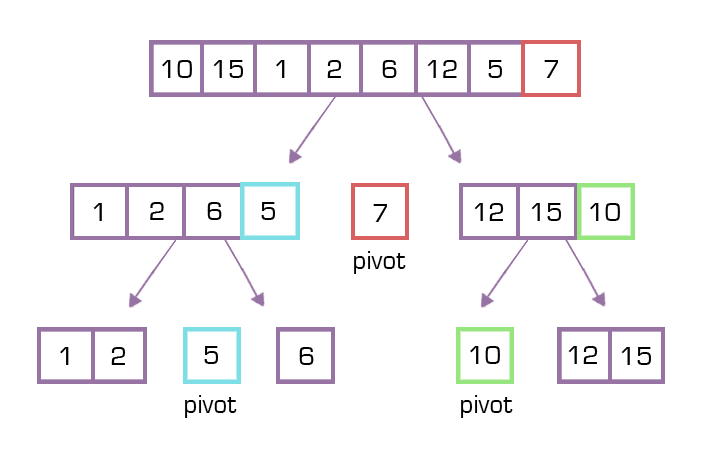
\includegraphics[width=\linewidth]{resources/quicksort.png}
        \caption{Illustration de l'algorithme de tri rapide}
    \end{figure}
    Complétez le code suivant:
    \lstinputlisting[language = python]{resources/quicksort.py}
    \begin{conseil}
        Pour le choix de votre élément pivot, pensez à utiliser la méthode \lstinline{randint()} de la librairie \lstinline{random}.
    \end{conseil}


    \begin{solution}
        \lstinputlisting[language = python]{solutions/quicksort_solution.py}
    \end{solution}
     


\end{Exercice}

\newpage
\section{Treap}
\begin{Exercice}[30 minutes]\textbf{Insertion dans un Treap: Python et Papier}\\
    Un arbre binaire de recherche montre de meilleures performances lorsqu'il est équilibré. Ainsi, la complexité d'une opération de recherche, d'insertion ou de suppression d'un nœud dans l'arbre équilibré \textit{a} est de $O(log n)$. Cette complexité est de $O(n)$ dans l'arbre \textit{b}.

    \begin{figure}[h]
        \centering
        \subfigure[Arbre équilibré]{
        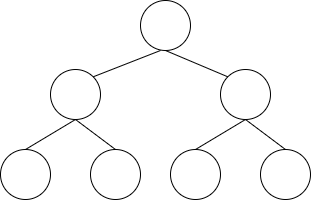
\includegraphics[width=.3\textwidth]{resources/binary_tree.png}
        }
        \subfigure[Arbre non équilibré]{
        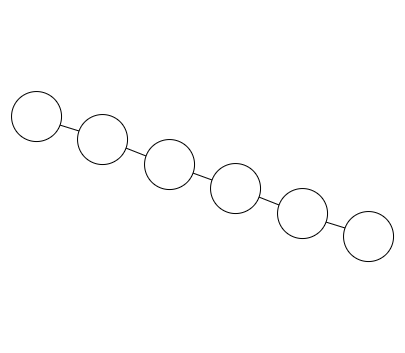
\includegraphics[width=.3\textwidth]{resources/linked_tree.png}
        }
        \caption{Exemple d'arbres binaires de recherche}
        \label{fig:architecture}
    \end{figure}

    Afin de s'assurer d'obtenir un arbre binaire de recherche presque équilibré, on peut utiliser les propriétés d'un Heap (ou tas) dont les éléments sont ordonnés en suivant une priorité. Dans un Max-heap (Figure~\ref{fig:maxheap}), le nœud ayant la priorité maximale se trouve toujours au sommet de l'arbre. Les nœuds parents auront toujours une priorité plus grande que les nœuds enfants. Dans un Min-heap tel que présenté en cours, le nœud ayant la plus faible priorité se trouve au sommet et dans cette configuration, les nœuds parents auront toujours une priorité plus petite que les nœuds enfants.

    \begin{figure}[h]
        \centering
        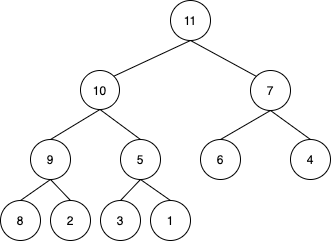
\includegraphics[width=.38\textwidth]{resources/heap.png}
        \caption{Exemple de Max-heap}
        \label{fig:maxheap}
    \end{figure}

    Un Treap (ou arbretas) est une fusion entre un arbre binaire de recherche et un Heap. En construisant un Treap, vous devez vous assurer que les deux conditions ci-dessous soient respectées:

    \begin{itemize}
        \item Le nœud de gauche a une valeur plus petite que le nœud parent, tandis que le nœud de droite a toujours une valeur plus grande que le nœud parent. --\textit{propriété d'un arbre binaire de recherche}
        \item Chaque enfant a une priorité plus petite que la priorité du parent. --\textit{propriété d'un max-heap}
    \end{itemize}

    Lors de l'insertion dans un Treap, si un nœud ne respecte pas les propriétés édictées ci-dessus, on procède à une rotation en permutant la position du nœud avec celle de son parent jusqu'à ce qu'on obtienne un Treap.

 
    Soit la liste suivante:

    \lstinline{liste = [5, 2, 1, 4, 9, 8, 10]}

    Dans le fichier \lstinline{treap.py} se trouvant sur Moodle, créer une nouvelle liste \lstinline{nodes} qui contient des ensembles de tuples à deux éléments. Chaque tuple contiendra un élément de \lstinline{liste} et une valeur aléatoire (comprise entre 0 et 99) représentant une priorité.

    Notez ci-dessous les valeurs que vous obtiendrez:\\ 

    {\Large
    nodes = [(5, ...), (2, ...), (1, ...), (4, ...), (9, ...), (8, ...), (10, ...)]\\}

    \begin{comment}
        Un Treap est un arbre binaire où chaque sommet $v$ a 2 valeurs, une clé \lstinline{v.key} et une priorité \lstinline{v.priority}. Un treap est une combinaison d'un arbre de recherche binaire et d'un heap.
        Un heap ou \emph{tas} est un arbre binaire presque complet (tous les niveaux sont remplis sauf, éventuellement, le dernier) dont les éléments sont ordonnés.
        Ainsi, le treap a la même structure qu'un arbre de recherche binaire dont les nœuds sont
        insérés par ordre de priorité. \\

        \lstinputlisting[language = python]{resources/treap.py}
    \end{comment}

    Placez les éléments de \lstinline{nodes} dans un Treap. Utilisez l'espace ci-dessous pour dessiner le Treap qui sera obtenu.


    \begin{conseil}
        \begin{itemize}
            \item Commencez d'abord par construire un arbre binaire de recherche en utilisant uniquement les clés, ensuite utilisez les priorités pour réorganiser les nœuds de votre arbre.
            \item Une fois complété, le programme \lstinline{treap.py} se trouvant sur Moodle générera un Treap en tenant compte de la position des éléments. 
            \item Utilisez la fonction \lstinline{random.randrange(100)} pour générer des nombres aléatoires compris entre 0 et 99.
            \item La propriété du Heap à satisfaire est que la priorité de la racine doit toujours être plus grande que celle de ses nœuds enfants.
            Les méthodes \lstinline{left_rotate} et \lstinline{right_rotate} permettent de réarranger les nœuds de façon à ce que la propriété du Heap soit satisfaite. Vous pouvez vous référer à l'illustration ci-dessous pour avoir une idée de comment fonctionnent les rotations.
            \begin{center}
                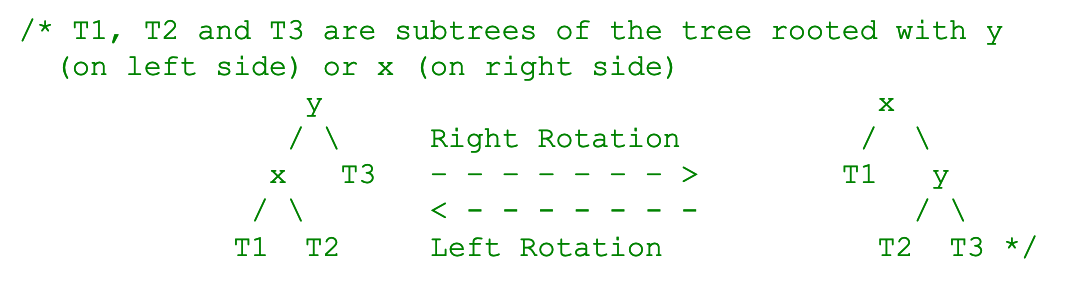
\includegraphics[width=\linewidth]{resources/treap_heap_property.png}
            \end{center}
        
        \end{itemize}
        
        
    \end{conseil}

    \begin{dessin}{}
        \vspace{14cm}
    \end{dessin}

    \begin{solution}
        \textbf{Code:}
        \lstinputlisting{solutions/treap.py}

    \textbf{\\Treap obtenu:} \\
    \lstinline{[(4,94), [(1,66), None, [(2,1), None, None]], [(10,30), [(5,26), None, [(8,20), None, [(9,4), None, None]]], None]]}

    \begin{center}
        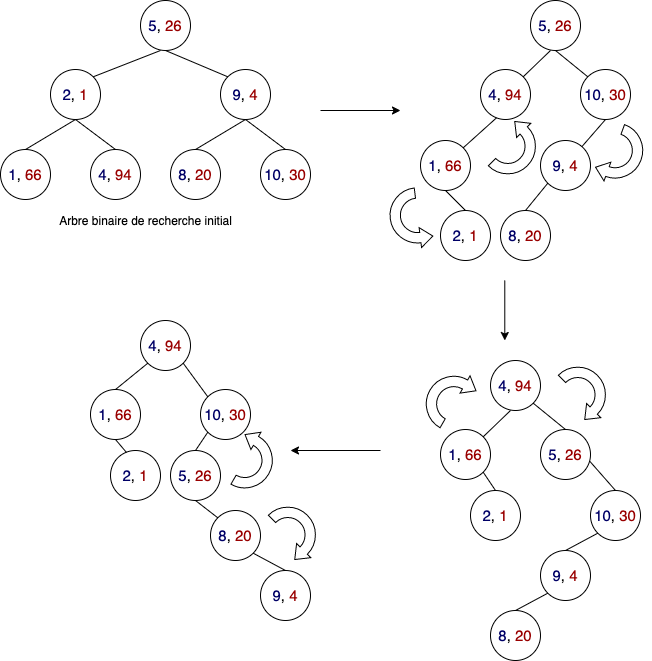
\includegraphics[width=\linewidth]{solutions/treap.png}
    \end{center}    
    \end{solution}
\end{Exercice}


\end{document}
